% X（旧 Twitter）投稿用の2段組版（A4 最大 4 ページ）。詳しくは main.tex。
\documentclass[a4paper,twocolumn,10pt]{ltjsarticle}
\usepackage[top=8mm,bottom=9mm,left=9mm,right=9mm,columnsep=6mm]{geometry}
\usepackage{amsmath,amssymb}
\usepackage{graphicx}
\usepackage{booktabs}
\usepackage{tabularx}
\usepackage{siunitx}
\usepackage{listings}
\usepackage{xcolor}
\usepackage[hidelinks]{hyperref}
\usepackage{enumitem}
\usepackage{caption}
\usepackage{subcaption}
\usepackage{titlesec}
\captionsetup{font=small,skip=2pt}
\setlist{itemsep=0pt,topsep=1pt,parsep=0pt,leftmargin=1.1em}
\titleformat{\section}{\large\bfseries\sffamily}{\thesection}{0.5em}{}
\titlespacing*{\section}{0pt}{5pt plus 1pt}{2pt}
\titleformat{\subsection}{\normalsize\bfseries\sffamily}{\thesubsection}{0.5em}{}
\titlespacing*{\subsection}{0pt}{3pt plus 1pt}{1pt}
\sisetup{detect-all}
\pagestyle{empty}
\setlength{\parskip}{0pt}
\setlength{\textfloatsep}{6pt plus 2pt minus 2pt}
\setlength{\floatsep}{4pt plus 1pt minus 1pt}
\setlength{\dbltextfloatsep}{6pt plus 2pt minus 2pt}
\setlength{\intextsep}{4pt plus 1pt minus 1pt}
\newcommand{\figref}[1]{図~\ref{#1}}
\newcommand{\tabref}[1]{表~\ref{#1}}
\newcommand{\lstref}[1]{リスト~\ref{#1}}
\newcommand{\code}[1]{\texttt{#1}}

\definecolor{lstbg}{gray}{0.955}
\lstset{
  basicstyle=\ttfamily\fontsize{6.3}{7.3}\selectfont,
  backgroundcolor=\color{lstbg}, frame=single, rulecolor=\color{gray!60},
  breaklines=true, columns=fullflexible, keepspaces=true,
  xleftmargin=1pt, xrightmargin=1pt, aboveskip=3pt, belowskip=3pt,
  framesep=2pt
}
\renewcommand{\lstlistingname}{リスト}

\begin{document}
\twocolumn[{%
  \begin{center}
    {\LARGE\bfseries 「全部任せる」の一言からウェブゲーム公開まで\par}
    \vspace{1mm}
    {\normalsize Claude Code の ultracode モードによるマルチエージェント開発の事例報告\par}
    \vspace{0.5mm}
    {\normalsize 貝淵蒼馬\par}
  \end{center}
  \vspace{-1mm}
  \noindent\fbox{\parbox{\dimexpr\textwidth-2\fboxsep-2\fboxrule}{\small
    \textbf{要旨}\quad クレーンで吊ったボールを振って壁の向こうに止める研究コード（運動方程式と軌道最適化）から，
    ブラウザゲーム「\textbf{ゆらしてピタッ}」を作り Cloudflare で公開した．依頼は
    「この振り子の遊びでwebゲームアプリ作りたい．全てそっちに任せるから，最強に面白いゲームを作って．」の2文だけで，
    設計・実装・検証はすべて Claude Code に任せた．本稿はセッションの記録（会話ログ，ワークフローの台本，サブエージェントの実行ログ）から，
    どんなプロンプトでどんな工程を踏んだかを再構成した．
    開発の本体は約 14.4 時間で，\textbf{7本のワークフローが延べ 70 体のサブエージェントを動かし}，ツール呼び出しは 5,921 回，トークンは約 1,900 万だった．
    工程は「複数案と審査による設計」「契約と仮実装の先行」「ファイル所有権を分けた並列実装と独立レビュー」
    「人間らしいボットによる難易度調査」「粗探し・反証・修正の総点検」と進んだ．
    人の指示は公開までに約 10 回で，出来を最も変えたのは試遊の「難しすぎる」だった．
    公開日（約 12 時間）の API 要求は \textbf{23,505 件}，クリアの記録が届いた端末は少なくとも \textbf{2,342 台}だった．}}
  \vspace{1.5mm}
  \begin{center}
    \begin{minipage}{0.21\textwidth}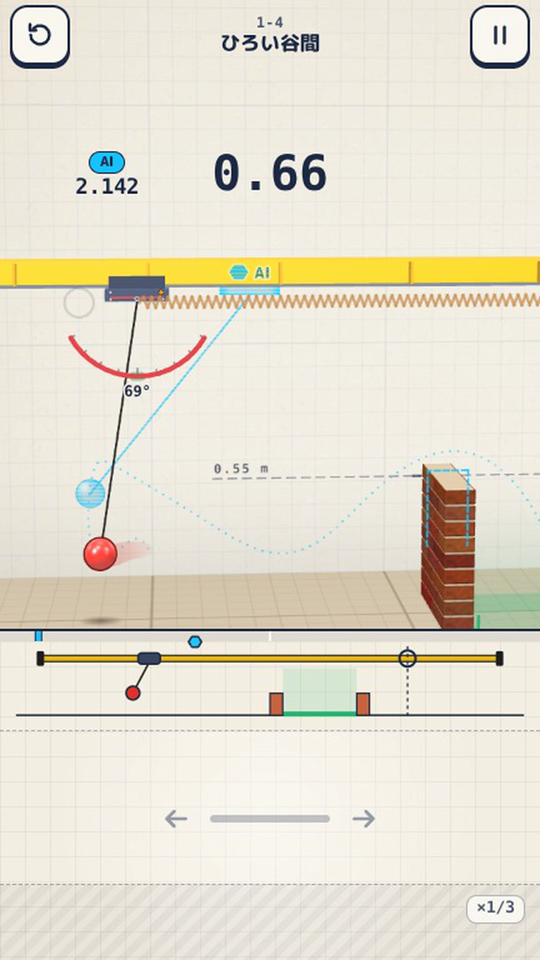
\includegraphics[width=\linewidth]{figs/shot_play.png}\end{minipage}\hfill
    \begin{minipage}{0.21\textwidth}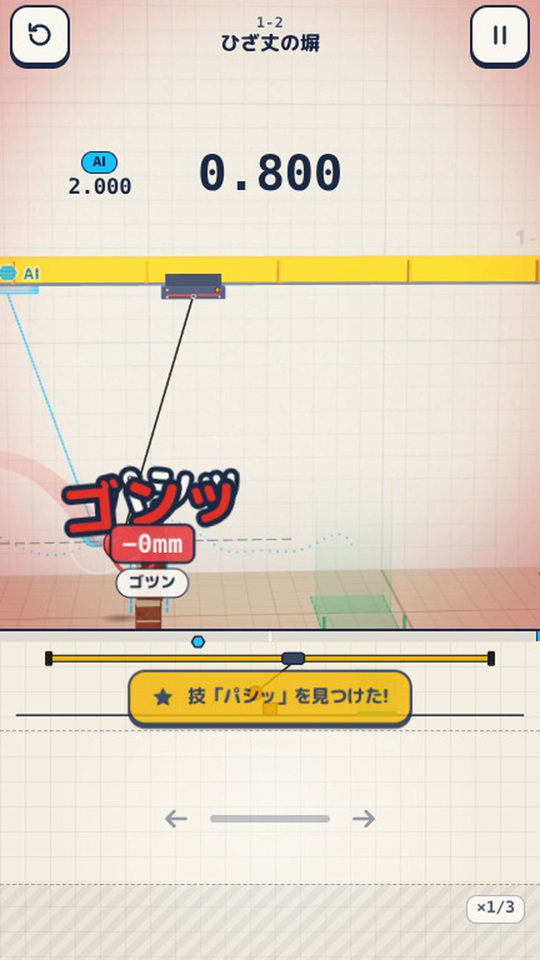
\includegraphics[width=\linewidth]{figs/shot_crash.png}\end{minipage}\hfill
    \begin{minipage}{0.21\textwidth}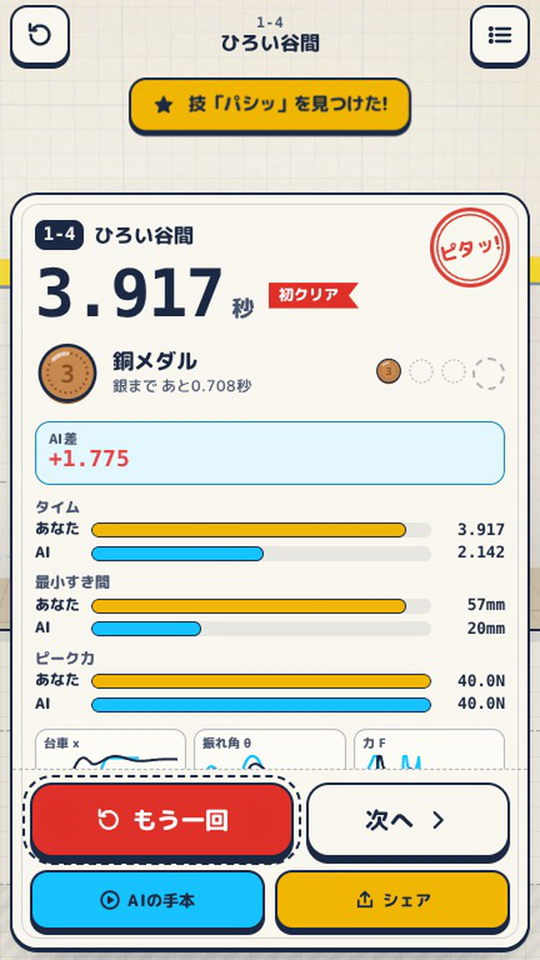
\includegraphics[width=\linewidth]{figs/shot_result.png}\end{minipage}\hfill
    \begin{minipage}{0.21\textwidth}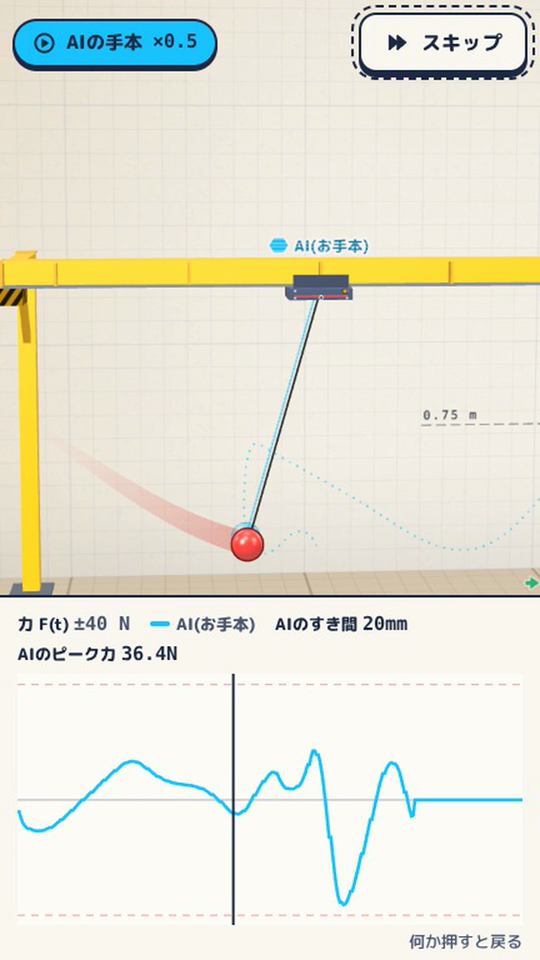
\includegraphics[width=\linewidth]{figs/shot_ai.png}\end{minipage}
    \captionof{figure}{完成したゲーム（実際のタッチ操作の録画から）．左から 1-4 のプレイ，1-2 で壁に激突，結果カード，2-2 の AI の手本と AI が掛けた力 $F(t)$．
    下半分が指で操作する盤，上の数字が AI と自分のタイム．}
    \label{fig:shots}
  \end{center}
  \vspace{1mm}
}]

\section{はじめに}
筆者は MathWorks のブログ記事\cite{gulley}の「クレーンで吊り荷を振って壁を越えさせる」問題を Python で再現し，
2枚の壁の間の隙間にボールを出し入れする問題へ広げた\cite{kaibuchi}．
台車 \SI{2}{kg} から \SI{1}{m} の紐で \SI{1}{kg} のボールを吊り，入力は台車を押す力（最大 \SI{40}{N}）だけである．
最短時間の軌道は CasADi/IPOPT で 1 問約 30 秒で解ける．
これを遊べる形にするため，\code{/effort ultracode} にしたうえで上記の2文だけを依頼した．
あえて大まかにしたのは，\textbf{全権を渡すと何ができるか}を調べたかったからである．
ultracode では Claude（以下，指揮役）がワークフロー（サブエージェント群を動かす JavaScript の台本）を自分で書いて走らせる．
モデルは開発が Opus 5，公開の段階は Opus 5.5 で，機械は 24 コアの Linux 1 台である．
本稿の引用プロンプトは台本の英語原文の抜粋である．

\begin{table}[t]
\centering
\caption{公開までに人が入れた指示（JST）}
\label{tab:human}
\footnotesize
\begin{tabularx}{\linewidth}{@{}l@{\hspace{3pt}}l@{\hspace{4pt}}X@{}}
\toprule
H1 & 9/22 13:47 & 最初の依頼（2文） \\
H2 & 13:56 & 「cloudflare で公開する予定だから，無料枠の範囲内で D1 とか割りと自由に使って」 \\
H3 & 17:52 & 「npm run dev のやり方とか教えて」 \\
H4 & 9/23 02:07 & 「CasADi 3.8.1 が js/WebAssembly に対応しているから，必要に応じて使ってね」 \\
H5 & 02:22 & 「キリがついたら Opus 5.5 で続けて」 \\
H6 & 09:43 & 再起動後「HANDOFF.md を読んで続きをやって」 \\
H7 & 10:55 & 試遊「\textbf{難しすぎる．減衰させようとすると加速する．矢印キーだけだと微調整がしづらすぎる}」 \\
H8 & 11:20頃 & 「日本語をデフォルトに」 \\
H9 & 11:42〜 & 公開手順の質問，起点日の選択，Cloudflare の画面操作 \\
H10 & 12:15〜 & 宣伝動画，コミット，GitHub Release \\
\bottomrule
\end{tabularx}
\end{table}

\section{工程の全体像}
開発セッションの流れを\figref{fig:gantt}，規模を\tabref{tab:wf}に示す．
\textbf{指揮役自身のツール呼び出しは 63 回だけ}で，残りはすべてサブエージェントが行った．
指揮役は台本を書き，結果を読み，次の台本に「決定事項」を書く役に徹した．
ツール呼び出しの大半は Bash（テスト，ビルド，シミュレーション，撮影）で，「動かして確かめる」に手数が使われていた．

\begin{figure*}[t]
\centering
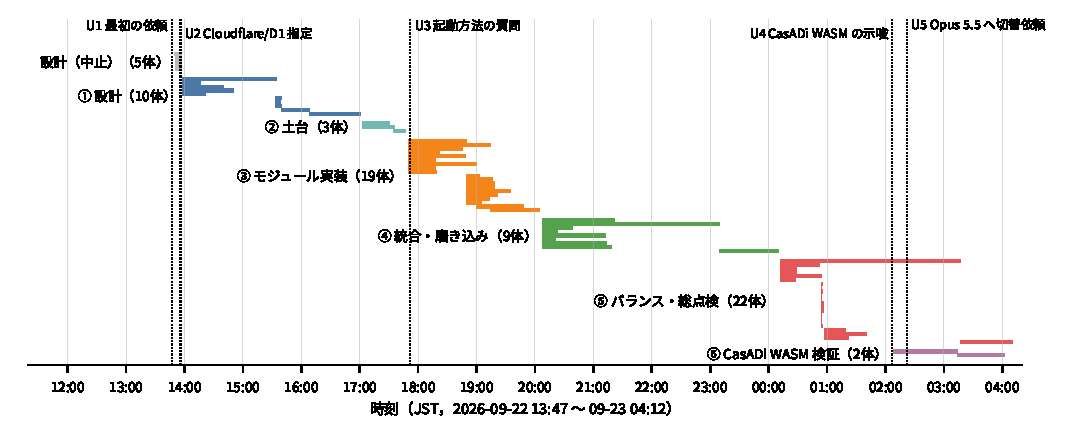
\includegraphics[width=0.96\textwidth]{figs/gantt_compact.pdf}
\caption{開発セッションでのサブエージェントの稼働（1本の横棒が1体）．点線 U1〜U5 は人の発言（\tabref{tab:human}の H1〜H5）．
設計（中止）は H2 を受けて止め，条件を差し替えてやり直したもの．}
\label{fig:gantt}
\end{figure*}

\begin{table}[t]
\centering
\caption{ワークフローごとの規模（時間は壁時計）}
\label{tab:wf}
\footnotesize
\begin{tabular}{@{}lrrrr@{}}
\toprule
ワークフロー & 体数 & 分 & ツール & トークン[万] \\
\midrule
設計（中止） & 5 & 6.5 & 29 & 39 \\
① 設計 & 10 & 183 & 330 & 208 \\
② 土台 & 3 & 45 & 240 & 84 \\
③ モジュール実装 & 19 & 135 & 2,351 & 784 \\
④ 統合・磨き込み & 9 & 242 & 1,399 & 332 \\
⑤ バランス・総点検 & 22 & 238 & 1,211 & 404 \\
⑥ CasADi WASM 検証 & 2 & 115 & 361 & 59 \\
\midrule
合計 & 70 & & 5,921 & 1,912 \\
\bottomrule
\end{tabular}
\end{table}

\section{各工程とプロンプト}

\subsection{① 設計：5案 → 3観点の審査 → 統合 → 批評}
全員に共通の前置きには，運動方程式，壁の寸法，最適化器の性能，公開条件が数値で書かれている．
H2 が届くと，指揮役は走行中の設計を止め，前置きを Cloudflare 無料枠（1日 10 万要求，1 要求 \SI{10}{ms} の CPU など）と
サーバー側の再計算による不正対策に書き換えてやり直した（\lstref{lst:ctx}）．

\begin{lstlisting}[float=t,caption={共通の前置き（H2 後に足された部分の抜粋）},label={lst:ctx}]
- Cheating: a public leaderboard will be attacked. ... the Worker re-simulates a submitted per-tick input log with
  the SAME TypeScript physics module ... This needs bit-exact cross-engine determinism (fixed timestep, inputs
  quantized per tick, own sin/cos implemented with + - * / only because Math.sin differs between V8/JavaScriptCore/
  SpiderMonkey) and must fit the 10 ms CPU budget ...
\end{lstlisting}

5体に別々の方向（mastery / arcade / campaign / mobile / sandbox）から1案ずつ作らせ，JSON スキーマで面の寸法まで書かせた．
審査役は「試遊責任者（楽しさ）」「主任エンジニア（作りやすさ）」「X でリンクを踏んで 30 秒しか我慢しない技術者（プレイヤー）」の3人で，
重み（楽しさ×2，最初の1分×1.5，作りやすさ×1.5，独自性，忠実さ）の合計は
mastery「ゆらしてピタッ／最適制御AIに，人間の指で勝て．」が 169.8 で首位，3人とも土台に選んだ．
他案からは「今日の5球」と Wordle 風の共有文，縦画面の操作盤，隙間を mm で見せる演出などが移植された．
一方，mobile 案の\textbf{「指を離すと LQR が揺れを止める」を中心に据えることは3人とも退けた}（「『ピタッ』を取り上げる」）．

統合役には「別々の AI エンジニアが話さずに並行して作れるほど正確に」と求め，約 2,300 行の設計書ができた．
続く批評役（``\textit{the lead engineer who must start building tomorrow}''）は最適化器を実際に走らせ，
解けない制限時間の面，D1 無料枠（1回 50 文）を超える送信，永久にランキングに載らない長い走行などを実装前に見つけて直した．

\subsection{② 土台：契約と仮実装を先に}
並列に入る前に，npm 一式，テスト基盤（Node，3ブラウザ，workerd，E2E），\textbf{全ファイルの型つき仮実装}を作り，全体が型チェックを通る状態にした．
物理のファイルに \code{Math.sin} を置くと lint が落ちることも実際に確かめさせた．
AI ゴーストは二分探索を省いた仮版を先に出し，本番（84 分）は裏で流した．最後に別の1体が全コマンドを自分で実行して検証した．

\subsection{③ 並列実装：所有権と独立レビュー}
物理・進行・入力・描画・音・UI・保存通信・Worker・日替わり生成の9担当を同時に動かした（\lstref{lst:rules}）．
各モジュールは作り終えると\textbf{物理コアの完成を待ってから}別のエージェントのレビューに回る．

\begin{lstlisting}[caption={並列実装の共通規則（抜粋）},label={lst:rules}]
- Only create/modify files you own ... If you need a change elsewhere, write it in your report
  (requests_for_other_owners).
- Never run git commands that change state. Never run npm install.
- If you run Playwright, ALWAYS set unique ports ...
- Quality bar: ... a genuinely fun, polished game (Nintendo-level feel), not a tech demo. Verify your work by
  actually running it (tests, builds, screenshots you look at with the Read tool). Report failures honestly.
\end{lstlisting}

描画担当には ``\textit{LOOK at your screenshots ... until the scene is genuinely attractive}''，
UI 担当には ``\textit{no purple gradients, no glassmorphism}'' と見た目の基準まで指定した．
全員が「受け入れ基準はすべて通過」と報告したが，レビューでは
レール端でボールが空中に止まる（物理），ボールに付く表示が本番に一つも出ていない（進行），
衝突音がスマホのスピーカーで鳴らない低域だった（音），2つ目のタブを閉じると進行が消える（保存）など，重大な不具合が次々に見つかった．

\subsection{④ 統合：決定事項と，人間らしいボット}
指揮役は各担当の「他担当への依頼」と「仕様からの逸脱」を裁定し，決定事項 D1〜D10 として次の台本の冒頭に置いた
（``\textit{LEAD DECISIONS (binding)}''）．同時に，人間らしいボットで難易度を調べさせた．
タッチは「折れ点 6 個以下・間隔 0.15 秒以上の折れ線」，キーは「切り替え 7 回以下」とし，
時刻 $\sigma=\SI{40}{ms}$・位置 $\sigma=\SI{1}{cm}$ のぶれを加えて成功率を測る．
結果，「たまご」は銅メダル不可能，5-2 は銅でも 9\%，キーボードは 2-2 を一度もクリアできないことがわかった．
統合役は実際のタッチとマウスで通しプレイを撮影し，押せないボタンなど 10 件を画像から見つけて直した．

\subsection{⑤ 総点検：粗探し → 反証 → 修正}
難易度を直す（壁を 5 cm ずらす，割れる張力を 16→18 N，キーは短押しで 5 cm，日替わり 84 面を解き直す）と並行して，
サーバー・物理・進行・見た目の4観点で読み取り専用の粗探しを行い，中・高の指摘は1件ずつ別の1体に反証させた（\lstref{lst:refute}）．

\begin{lstlisting}[caption={反証役へのプロンプト（全文）},label={lst:refute}]
# Role: skeptical verifier (read-only on the game source; ...)
Try to REFUTE this finding. Read the code paths involved, and if cheap, reproduce it with a small script/test.
Default to real=false if you cannot substantiate it. If real, give the right severity and the best fix.
\end{lstlisting}

指摘 26 件のうち中・高の 12 件が確定し（「高」3件はすべて「中」に格下げ），
他人のリプレイを使い回して上位 100 を埋められる，IPv6 の /64 から無制限に送れる，日替わり5球目の結果が消える，などを直した．
修正には回帰テストを付け，それが元のコードで落ちることまで確かめている．
最終的に単体 1,299・ブラウザ 80・E2E 262 件が通り，たまごの銅到達率は 0→32\%，5-2 は 9→35\% になった．
ただしキーボードの 2-2 は 1\% のままで，ゲート役は「失敗の 8〜9 割は壁への衝突」と原因を正しく報告していた．

\subsection{⑥ 人のヒントの検証と引き継ぎ}
H4 を受けた指揮役は，ゲームに触れない場所で2体に試させた．
JS に移した最適化問題は Python と目的関数がビット単位で一致し，ブラウザで 0.4〜0.5 秒で解き直せたが，
確認役が\textbf{同梱の METIS 4 のライセンスが再配布を禁じている}ことを見つけ，「いまは使わない」と判断した．
H5 では動作中の2本の終了を待ち，\code{HANDOFF.md} に現状と残作業をまとめてから再起動を依頼した．

\section{人の試遊と公開}
H7 を受けて，Opus 5.5 の指揮役は自分で原因を調べた．キーは 0.17 秒で最高速に達し，止めようとするたびに揺らしていた．
そこで\textbf{ゴールの 30 cm 以内で手を離すと離散時間 LQR が揺れを止める「ゆれ止めアシスト」}を入れ，
止まるまでの時間はパッド面で 15〜24 秒から 2〜3.6 秒になった．記録は力の列のままなので，サーバー検証も使える．
これは①で3人の審査役が退け，設計書では最低優先度の補助に置かれていた案とほぼ同じものである．
人が遊ぶと，それなしでは難しすぎた．結果として既定でオン，ランキング対象で出荷した．

公開では，外部に影響する操作を人に委ねた．公開後に変えられない日替わりの起点日を選択肢で尋ね，
まっさらな状態からのビルドを確かめてから push し，Cloudflare の画面操作は手順を示して人が行った．
公開は 9/23 11:59．続けて，シミュレーターで「クリアできる指の動き」を探してから実機操作を録画し，
VOICEVOX と Remotion で 27.6 秒の宣伝動画を作った．

\section{規模と反響}
設計段階では「5〜15k 行でよい」としていたが，テスト込みで約 5.5 万行（うちテスト 1.9 万）になった．
18 面すべてに最適化器の AI ゴーストがあり，日替わり 84 面も最適化器で解いてある．
物理は自前の sin/cos で Chromium・Firefox・WebKit・workerd の結果がビット単位で一致し，
Worker が送られた入力列を同じ物理で再計算してランキングを検証する．音はすべて WebAudio の合成，外部素材はない．

\begin{table}[t]
\centering
\caption{公開日（9/23 JST，約 12 時間）の反響．上3行は Cloudflare の分析 API，下2行は本番 D1（9/24 00:24 時点）}
\label{tab:reception}
\footnotesize
\begin{tabular}{@{}lr@{}}
\toprule
Worker 実行（\code{/api/*}，エラー 0） & \textbf{23,505} \\
\quad 最多の 1 時間（16 時台） & 4,364 \\
静的ファイル配信（99.5\% キャッシュ） & 24,673 \\
クリアが届いた端末（重複なし） & \textbf{2,342} \\
1-1 / 1-2 / 1-3 / 1-4 をクリアした端末 & 1,729 / 1,264 / 1,044 / 633 \\
\bottomrule
\end{tabular}
\end{table}

\texttt{workers.dev} で公開しているので訪問者数そのものは取れず，端末数は\textbf{クリアの記録が届いた端末の下限}である
（記録用の表は当日 20:44 に追加し，それ以前は上位 100 位か AI に勝った走行しか残っていない）．
Worker 実行は無料枠（1日 10 万）の約 24\% で，設計時の「1日 2 万人でも無料枠内」の見積もりに収まっている．

\section{考察}
\textbf{完成度を上げた工夫}を役割ごとにまとめる．
\begin{itemize}
  \item \textbf{判断を分ける}：5案を独立に作らせ3観点で採点．設計書は「話さずに並行開発できる精度」で書かせ，批評役に数値を測り直させた．
  \item \textbf{並行でも壊れない形}：契約と仮実装を先に作る．ファイル所有者は1人．依頼は報告経由．ポートと出力先を担当ごとに分ける．重い計算は仮版を先に．
  \item \textbf{自己申告を信用しない}：作る役と確かめる役を必ず分け，反証役は「裏付けがなければ偽」．修正には元のコードで落ちる回帰テスト．「テストを弱めるな」を繰り返す．
  \item \textbf{目で見て，遊ばせる}：スクリーンショットを画像として読んで直す．人間らしい制約とぶれをもつボットに遊ばせて数値で測る．
\end{itemize}
\textbf{人が必要だったところ}：人の指示は約 10 回で，大半は公開先と公開操作だった．
出来を最も変えたのは H7 で，審査役は「ピタッは腕の見せ所」を重く見て自動制御を補助に下げ，
ボットはキーボードの弱点を数値で示したが直しきれなかった．指揮役自身も「ボットでは画面を見ながら指で調整する感じまでは再現できない」と書いていた．
外部に影響する操作は必ず人に確認し，人のヒント（CasADi）も鵜呑みにせず検証してから見送った．

\textbf{費用と限界}：70 体・約 1,900 万トークンは趣味の開発には大きい．工程の長さは最適化器の計算（本番ゴースト 84 分，日替わりの解き直し約 2.7 時間）で決まっていた．
また本稿の分析と執筆も Claude Code が行っており，「工夫」の選び方には作った側の視点が入りうる．

\begin{thebibliography}{9}
\setlength{\itemsep}{0pt}
\footnotesize
\bibitem{gulley} N.~Gulley, ``Simulate in MATLAB, Animate in Blender,'' MathWorks Blogs, 2026.
\bibitem{kaibuchi} 貝淵蒼馬，「吊り下げボールを壁の隙間に出し入れするガントリークレーン」，\url{https://github.com/Raptor-zip/crane-ball-wall}．
\end{thebibliography}

\end{document}
